% Chapter 10, Section 4

\section{Gated Recurrent Units (GRU) \difficultyInline{intermediate}}
\label{sec:gru}

\subsection*{Intuition}

GRU simplifies LSTM by merging cell and hidden state and combining gates, often matching performance with fewer parameters—useful when data or compute is limited \cite{Cho2014,GoodfellowEtAl2016}.

\subsection*{Historical Context}

Proposed in the mid-2010s, GRU offered a practical alternative to LSTM with competitive empirical results and simpler implementation \cite{Cho2014}.

% Index and glossary
\index{gated recurrent unit}
\glsadd{recurrent-neural-network}

\subsection{Architecture}

GRU simplifies LSTM with fewer parameters and merges the cell and hidden state into a single vector, often yielding comparable performance with less computation \cite{Cho2014,GoodfellowEtAl2016}:

\begin{align}
\vect{z}_t &= \sigma(\mat{W}_z [\vect{h}_{t-1}, \vect{x}_t]) \quad \text{(update gate)} \\
\vect{r}_t &= \sigma(\mat{W}_r [\vect{h}_{t-1}, \vect{x}_t]) \quad \text{(reset gate)} \\
\tilde{\vect{h}}_t &= \tanh(\mat{W} [\vect{r}_t \odot \vect{h}_{t-1}, \vect{x}_t]) \quad \text{(candidate)} \\
\vect{h}_t &= (1 - \vect{z}_t) \odot \vect{h}_{t-1} + \vect{z}_t \odot \tilde{\vect{h}}_t
\end{align}

\subsection{Architecture (visual)}
\begin{figure}[h]
    \centering
    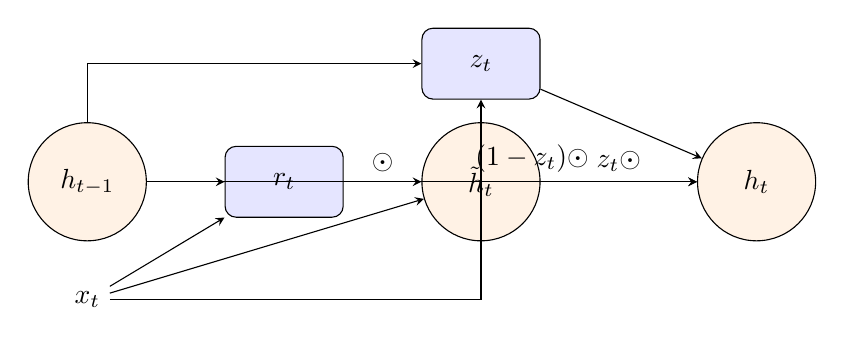
\begin{tikzpicture}[>=stealth, node distance=2.0cm]
        \tikzstyle{gate}=[draw, rounded corners, minimum width=1.5cm, minimum height=0.9cm, fill=blue!10]
        \tikzstyle{state}=[draw, circle, minimum width=1.5cm, fill=orange!10]
        
        % Previous hidden state
        \node[state] (ht1) {$\vect{h}_{t-1}$};
        
        % Input
        \node[below of=ht1, yshift=0.5cm] (xt) {$\vect{x}_t$};
        
        % Reset gate
        \node[gate, right of=ht1, xshift=0.5cm] (rt) {$\vect{r}_t$};
        
        % Candidate hidden state
        \node[state, right of=rt, xshift=0.5cm] (cand) {$\tilde{\vect{h}}_t$};
        
        % Update gate
        \node[gate, above of=cand, yshift=-0.5cm] (zt) {$\vect{z}_t$};
        
        % Current hidden state
        \node[state, right of=cand, xshift=1.5cm] (ht) {$\vect{h}_t$};
        
        % Arrows
        \draw[->] (ht1) -- (rt);
        \draw[->] (xt) -- (rt);
        \draw[->] (xt) -| (zt);
        \draw[->] (ht1) |- (zt);
        \draw[->] (rt) -- node[midway, above] {$\odot$} (cand);
        \draw[->] (xt) -- (cand);
        \draw[->] (cand) -- node[midway, above] {$\vect{z}_t \odot$} (ht);
        \draw[->] (ht1) -- node[pos=0.7, above] {$(1-\vect{z}_t) \odot$} (ht);
        \draw[->] (zt) -- (ht);
    \end{tikzpicture}
    \caption{GRU architecture showing update gate $\vect{z}_t$, reset gate $\vect{r}_t$, and information flow from $\vect{h}_{t-1}$ and $\vect{x}_t$ to $\vect{h}_t$.}
    \label{fig:gru_architecture}
\end{figure}

\subsection{Comparison with LSTM}
\begin{table}[h]
    \centering
    \begin{tabular}{@{}p{3.2cm}p{5.2cm}p{5.2cm}@{}}
    \toprule
    & \textbf{GRU} & \textbf{LSTM} \\
    \midrule
    State & Single hidden state $\vect{h}_t$ & Hidden $\vect{h}_t$ and cell $\vect{c}_t$ \\
    Gates & Update, reset & Input, forget, output \\
    Parameters & Fewer (often faster) & More (more expressive) \\
    Long-range deps. & Good in practice & Often stronger on very long spans \\
    Simplicity & Simpler to implement & Slightly more complex \\
    Typical use & Smaller data/compute budgets & Longer sequences or when capacity helps \\
    \bottomrule
    \end{tabular}
    \caption{GRU vs. LSTM at a glance \cite{Cho2014,Hochreiter1997,GoodfellowEtAl2016}.}
\end{table}

The choice between GRU and LSTM often depends on the specific task requirements and computational constraints. GRU's simpler architecture with fewer parameters makes it computationally more efficient, typically requiring less memory and allowing for faster training, which can be particularly advantageous when working with limited computational resources or when rapid prototyping is needed. Empirically, GRU performance is often comparable to LSTM on many tasks, especially those with moderate sequence lengths, though LSTM tends to have a slight edge on problems requiring very long-term dependencies due to its separate cell state that can maintain information more independently. In practice, both architectures have proven highly effective, and the choice often comes down to experimentation—trying both on your specific dataset and choosing the one that yields better validation performance whilst considering training time and deployment constraints. Modern deep learning frameworks make it straightforward to swap between these architectures, so practitioners can easily evaluate both options during model development.

